\section{Конформні відображення: загальні положення і приклади}

\subsection{Поняття конформного відображення}

Припустимо, що задано неперервне і взаємно-однозначне відображення області $D$ на область $D^\star$:
\begin{equation}
    \label{eq:27.1}
    w = f(z) = u(x, y) + i v(x, y).
\end{equation}

Припустимо також, що функції $u(x, y)$ і $v(x, y)$ диференційовні в цій області. \\

Зафіксуємо довільну точку $z_0$ з $D$ і в її околі замінимо прирости функцій $u$ і $v$ диференціалами. \\

За визначенням диференціала, приріст представляється у вигляді
\begin{equation}
    \label{eq:27.2}
    \left\{
        \begin{aligned}
            u - u_0 &= \dfrac{\partial u}{\partial x} \cdot (x - x_0) + \dfrac{\partial u}{\partial y} \cdot (y - y_0) + \eta_1 \Delta r, \\
            v - v_0 &= \dfrac{\partial v}{\partial x} \cdot (x - x_0) + \dfrac{\partial v}{\partial y} \cdot (y - y_0) + \eta_2 \Delta r,
        \end{aligned}
    \right.
\end{equation}
де частинні похідні беруться у точці $z_0$, $\Delta r = \sqrt{(x - x_0)^2 + (y - y_0)^2}$, а $\eta_1, \eta_2 \to 0$ при $\Delta r \to 0$. \\

Заміна приростів диференціалами зводиться до відкидання у співвідношеннях \LaReF{eq:27.2} членів $\eta_1 \Delta r$ і $\eta_2 \Delta r$, які є о-малими у порівнянні з іншими членами цих співвідношень якщо припустити, що 
\begin{equation*}
    \left( \dfrac{\partial u}{\partial x} \right)^2 + \left( \dfrac{\partial u}{\partial y} \right)^2 \ne 0, \quad \left( \dfrac{\partial v}{\partial x} \right)^2 + \left( \dfrac{\partial v}{\partial y} \right)^2 \ne 0.
\end{equation*}

Геометрично ця заміна рівносильна заміні відображенння $w = f(z)$ відображенням
\begin{equation}
    \label{eq:27.3}
    \left\{
        \begin{aligned}
            u - u_0 &= \dfrac{\partial u}{\partial x} \cdot (x - x_0) + \dfrac{\partial u}{\partial y} \cdot (y - y_0), \\
            v - v_0 &= \dfrac{\partial v}{\partial x} \cdot (x - x_0) + \dfrac{\partial v}{\partial y} \cdot (y - y_0),
        \end{aligned}
    \right.
\end{equation}
яке називається головною лінійною частиною відображення \LaReF{eq:27.1}. \\

Відображення \LaReF{eq:27.3} можна переписати у вигляді
\begin{equation}
    \label{eq:27.4}
    \left\{
        \begin{aligned}
            u &= a x + b y + l, \\
            v &= c x + d y + m,
        \end{aligned}
    \right.
\end{equation}
де
\begin{equation}
    \label{eq:27.5}
    \left\{
        \begin{aligned}
            a = \dfrac{\partial u}{\partial x}, \quad b = \dfrac{\partial u}{\partial y}, &\quad c = \dfrac{\partial v}{\partial x}, \quad d = \dfrac{\partial v}{\partial y}, \\
            l = u_0 - \dfrac{\partial u}{\partial x} \cdot x_0 - \dfrac{\partial u}{\partial y} \cdot y_0, &\quad m = v_0 - \dfrac{\partial v}{\partial x} \cdot x_0 - \dfrac{\partial v}{\partial y} \cdot y_0
        \end{aligned}
    \right.
\end{equation}
не залежать від $x$ і $y$. \\

Воно являє собою так зване лінійне перетворення площини $(x, y)$. \\

Згадаємо основні властивості лінійних перетворень. \\

Кожне лінійне перетворення \LaReF{eq:27.4} однозначно визначене у всій площині $z$. \\

У припущенні $\Delta = a d - b c \ne 0$, обернене до \LaReF{eq:27.4} перетворення
\begin{equation}
    \label{eq:27.6}
    \left\{
        \begin{aligned}
            x &= \dfrac 1 \Delta \cdot (d u - b v - d l + b m), \\
            y &= \dfrac 1 \Delta \cdot (- c u + a v + lc - a m)
        \end{aligned}
    \right.
\end{equation}
також однозначно визначене у всій площині $w$. \\

Таким чином, при $\Delta \ne 0$ не тільки кожному значенню $z$ відповідає єдине значення $w$ але і кожному значенню $w$ -- єдине значення $z$, тобто перетворення \LaReF{eq:27.4} реалізує взаємно-однозначне відображення всієї площини $z$ на всю площину $w$. \\

Розглянемо пучок паралельних прямих із кутовим коефіцієнтом $k = \tan \phi$, тобто прямих $y = k x + C$. \\

Замінюючи $x$ і $y$ за формулами \LaReF{eq:27.6} бачимо, що цьому пучку відповідає пучок паралельних прямих 
\begin{equation*}
    -c u + a v + l c - a m = k \cdot (d u - b v - d l + b m) + C \cdot \Delta
\end{equation*} 
з кутовим коефіцієнтом 
\begin{equation*}
    k^\star = \tan \theta = \dfrac{c + k d}{a + k b}.    
\end{equation*}

Тобто відображення \LaReF{eq:27.4} перетворює квадрати у площині $z$ в паралелограми у площині $w$. \\

Нехай $z_0 = x_0 + i y_0$ і $w_0 = u_0 + i v_0$ -- пара точок, які відповідають одна одній при відображення \LaReF{eq:27.4}. \\

Тоді це відображення можна представити у вигляді
\begin{equation}
    \label{eq:27.7}
    \left\{
        \begin{aligned}
            u - u_0 &= a \cdot (x - x_0) + b \cdot (y - y_0), \\
            v - v_0 &= c \cdot (x - x_0) + d \cdot (y - y_0), 
        \end{aligned}
    \right.
\end{equation}
а обернене перетворення -- у вигляді
\begin{equation}
    \label{eq:27.8}
    \left\{
        \begin{aligned}
            x - x_0 &= \dfrac d \Delta \cdot (u - u_0) - \dfrac b \Delta \cdot (v - v_0), \\
            y - y_0 &= - \dfrac c \Delta \cdot (u - u_0) + \dfrac a \Delta \cdot (v - v_0).
        \end{aligned}
    \right.
\end{equation}

Враховуючи формули \LaReF{eq:27.8}, ми можемо стверджувати, що кола з центром у точці $z_0$:
\begin{equation*}
    (x - x_0)^2 + (y - y_0)^2 = r^2,
\end{equation*}
при відображення \LaReF{eq:27.4} переходять у еліпси з центром в точці $w_0$:
\begin{equation}
    \label{eq:27.9}
    (d^2 + c^2) \cdot (u - u_0)^2 - 2 (b d + a c) \cdot (u - u_0) \cdot (v - v_0) + (b^2 + a^2) \cdot (v - v_0)^2 = \Delta^2 r^2.
\end{equation}

Знайдемо умови на коефіцієнти перетворення \LaReF{eq:27.4} необхідні і достатні для того, щоб воно переводило кола в кола. \\

Із співвідношень \LaReF{eq:27.9} випливає, що для цього необхідно і достатньо виконання співвідношень
\begin{equation}
    \label{eq:27.10}
    b d + a c = 0, \quad a^2 + b^2 = c^2 + d^2.
\end{equation}

Перше з них дає $a = \lambda d$, $b = -\lambda c$, причому підставляючи це у друге рівняння з \LaReF{eq:27.10} отримаємо, що $\lambda = \pm 1$. \\

Випадок $\lambda = 1$ приводить до співвідношень
\begin{equation}
    \label{eq:27.11}
    a = d, \quad b = -c.
\end{equation}

У цьому випадку $\Delta = a d - b c = a^2 + b^2 > 0$. \\

Оскільки 
\begin{equation*}
    \left( \dfrac{a}{\sqrt{\Delta}} \right)^2 + \left( \dfrac{b}{\sqrt{\Delta}} \right)^2 = \dfrac{a^2 + b^2}{\Delta} = 1,
\end{equation*}
то можемо покласти
\begin{equation*}
    a = d = \sqrt{\Delta} \cdot \cos \alpha, \quad c = - b = \sqrt{\Delta} \cdot \sin \alpha,
\end{equation*}
тоді \LaReF{eq:27.4} перепишеться у вигляді
\begin{equation*}
    u = \sqrt{\Delta} \cdot (\cos \alpha \cdot x - \sin \alpha \cdot y) + l, \quad v = \sqrt{\Delta} \cdot ( \sin \alpha \cdot x + \cos \alpha \cdot y) + m.
\end{equation*}

Ці співвідношення можна записати к комплексній формі наступним чином:
\begin{equation*}
    u + i v = \sqrt{\Delta} \cdot (\cos \alpha + i \sin \alpha) \cdot (x + i y) + l + i m,
\end{equation*}
і вони приводяться до лінійної функції комплексної змінної 
\begin{equation}
    \label{eq:27.12}
    w = A z + B,
\end{equation}
де 
\begin{equation}
    \label{eq:27.13}
    A = \sqrt{\Delta} \cdot e^{i \alpha}, \quad B = l + i m.
\end{equation}

Звідси видно, що при умовах \LaReF{eq:27.11} лінійне перетворення \LaReF{eq:27.4} зводиться до зсуву площини $z$ на вектор $B = l + i m$, повороту на кут $\alpha = \Arg A$ і розтягненню з коефіцієнтом $\sqrt{\Delta} = |A|$. \\

У випадку $\lambda = -1$ ми маємо:
\begin{equation}
    \label{eq:27.14}
    a = - d, \quad b = c
\end{equation}
і $\Delta = - a^2 - b^2 < 0$. Повторюючи, що тільки проведені викладки, побачимо, що перетворення \LaReF{eq:27.4} можна записати так:
\begin{equation}
    \label{eq:27.15}
    q = \sqrt{-\Delta} \cdot e^{i \alpha} \cdot \overline{z} + B.
\end{equation}
Як наслідок, за умов \LaReF{eq:27.14} до перерахованих вище перетворень додається ще перехід від $z$ до $\overline{z}$, тобто симетрія відносно дійсної вісі. \\

З геометричного сенсу перетворень \LaReF{eq:27.12} і \LaReF{eq:27.15} зрозуміло, що вони зберігають кути між прямими. Таким чином, умови \LaReF{eq:27.10} є умовами ортогональності. Причому \LaReF{eq:27.12} зберігає орієнтацію, а \LaReF{eq:27.15} її змінює. \\

Повернемося до довільних відображень. Взаємно-однозначне відображення 
\begin{equation}
    \label{eq:28.1}
    w = f(z) = u(x, y) + i v(x, y)
\end{equation}
області $D$ на область $D^*$ називається \textit{конформним} якщо в околі довільної точки $D$ головна лінійна частина цього відображення є ортогональним перетворенням, яке зберігає орієнтацію. З цього визначення випливають основні властивості конформних відображень:
\begin{enumerate}
    \item конформне відображення перетворює нескінченно малі кола в нескінченно малі кола;
    \item конформне відображення зберігає кути між кривими в точках їх перетину.
\end{enumerate}
\begin{figure}[H]
    \centering
    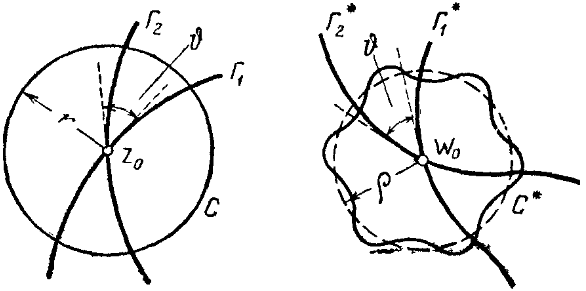
\includegraphics[scale=.5]{mal-38.png}
    \caption{дія конформного відображення на нескінченно малі кола}
    \label{fig:38}
\end{figure}

Враховуючи формули \LaReF{eq:27.5} і \LaReF{eq:27.11} ми можемо записати умови конформності відображення \LaReF{eq:28.1} у вигляді
\begin{equation}
    \label{eq:27.16}
    \dfrac{\partial u}{\partial x} = \dfrac{\partial v}{\partial y}, \quad \dfrac{\partial u}{\partial y} = - \dfrac{\partial v}{\partial x},
\end{equation}
причому
\begin{equation}
    \label{eq:27.17}
    \Delta = \left( \dfrac{\partial u}{\partial x} \right)^2 + \left( \dfrac{\partial v}{\partial x} \right)^2 = |f'(z_0)|^2 \ne 0,
\end{equation}
адже при $\Delta = 0$ головна лінійна частині відображення $w = f(z)$ вироджується, що суперечить умові конформності. Таким чином, умови конформності збігаються з умовами Коші-Рімана аналітичності функції $f(z)$ в області $D$, причому нерівність \LaReF{eq:27.17} показує, що похідна $f'(z)$ має бути всюди відмінною від нуля. \\

Далі маємо 
\begin{equation*}
    \dfrac{\partial u}{\partial x} = \dfrac{\partial v}{\partial y} = \sqrt{\Delta} \cdot \cos \alpha, \quad \dfrac{\partial v}{\partial x} = - \dfrac{\partial u}{\partial y} = \sqrt{\Delta} \cdot \sin \alpha,
\end{equation*}
звідки легко отримати геометричну інтерпретацію похідної від функції комплексної змінної. Справді, маємо
\begin{equation}
    \label{eq:27.18}
    |f'(z) = \sqrt{\Delta}; \quad \arg f'(z) = \alpha,
\end{equation}
тобто модуль і аргумент похідної $f'(z)$ позначають коефіцієнт розтягнення і кут повороту головної лінійної частини відображення $w = f(z)$ в точці $z$. \\

Резюмуючи, для того щоб функція $w = f(z)$ реалізувала конформне відображення області $D$ необхідно і достатньо, аби в цій області вона була однолистою, аналітичною, і щоб її похідна не перетворювалася на 0 (причому ця остання умова випливає з однолистості). \\

Наостанок, якщо функція аналітична але не однолиста в певній області, то все ще можна сказати, що вона реалізує конформне відображення у достатньо малих околах точок $z$ в яких $f'(z) \ne 0$. Точки ж у яких $f'(z) = 0$ а також їхні образи називаються точками гілкування.

% page 108 text = page 121 file, after equation (13)